\section*{Contexte du stage}
L’équipe Inria Mosaic du RDP à l’ENS de Lyon développe des modèles
mathématiques et numériques pour étudier la morphogenèse des plantes
et des animaux. Dans ce contexte elle est amenée à concevoir des
structures de données génériques et efficaces représenter
mathématiquement les formes modélisées. Pour représenter les systèmes
ramifiés des plantes par exemple, on a souvent recours à des
structures de données arborescentes. Ces dernières sont souvent très
lourdes en mémoire et peuvent entrainer des coûts algorithmiques
importants. Pour éviter cela, l’équipe a développé depuis quelques
années une méthode permettant de compresser de façon exacte ou
approchée les structures arborescentes, basée sur l’élimination des
structures redondantes. Cette méthode conduit à représenter les
structures arborescentes par des Graphes Orientés Acycliques (DAGs). On
peut montrer que les arborescences qui se compressent sous forme de
DAGs linéaires (DAGs hamiltoniens) ont les meilleurs taux de
compression. Ces arborescences sont dites “linéaires”.  Pour
compresser une arborescence quelconque, tout en tolérant une perte
d’information, il est donc envisageable de chercher l’arborescence
linéaire la plus proche d’une arborescence donnée et de compresser
cette dernière. Ceci peut s’exprimer formellement comme un problème
d’optimisation.

\section*{Expression formelle du problème d'optimistation}
Notons $\mathcal{T}$ l'ensemble des arbres non ordonnés (c'est-à-dire
que l'on ne considère pas d'ordre sur les fils d'un noeud).
Nous noterons par la suite $T[v]$ le sous-arbre de $T$ ayant $v$ pour racine.

Considérons la relation d'équivalence $\equiv$ sur $\mathcal{T}$
définie par $T_1 \equiv T_2$ si et seulement si $T_1$ et $T_2$ sont
isomorphes. Plus généralement, nous dirons que deux sommets $v_1$ et
$v_2$, de $T_1$ et $T_2$ respectivement, sont équivalents si les
sous-arbres $T_1[v_1]$ et $T_2[v_2]$ sont isomorphes. Nous noterons
$C(v)$ la classe d'équivalence de $v$.

Pour $T = (V,E) \in \mathcal{T}$, posons
$\mathcal{Q}(T) = (V_{\mathcal{Q}}, T_{\mathcal{Q}})$ le graphe obtenu
en quotientant les sommets de $T$ par la relation
$\equiv$. Concrêtement, $V_{\mathcal{Q}} = \{ C(v) | v \in V \}$ et
$E_{\mathcal{Q}} = \{ (C(u), C(v)) | (u,v) \in T \}$. Définissons
$\delta$ la fonction de pondération sur $\mathcal{Q}(T)$ définie par
$$\delta(C(u), C(v)) = \#\{ v' \in Fils(u) | C(v) = C(v')\}$$.

La figure \ref{fig:exemple} (tirée de \cite{godin}) représente un
arbre (à gauche) et son graphe quotient (à droite). Les sommets
équivalents sont représentés d'une même couleur.

\begin {figure} [h]
  \centering
  \subfloat{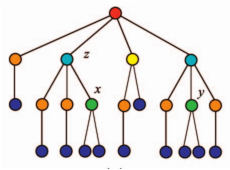
\includegraphics[width=.3\textwidth]{figures/fig1.pdf}}
  \subfloat{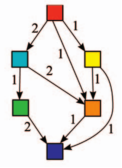
\includegraphics[width=.16\textwidth]{figures/fig2.pdf}}
  \caption{Exemple de graphe quotient}
  \label{fig:exemple}
\end{figure}

Pour tout $T \in \mathcal{T}$, $\mathcal{Q}(T)$ est un \emph{DAG} (un
graphe sans cycle orienté). De plus, pour tout \emph{DAG} $Q$, il
existe un unique $T \in \mathcal{T}$ tel que $\mathcal{Q}(T) =
Q$ \cite{godin}.

L'avantage de la représentation d'un arbre $T$ par son graphe quotient
$\mathcal{Q}(T)$ tient au fait que $\mathcal{Q}(T)$ est une
représentation compréssée. Par exemple, si une grandeur $f$ est
définie inductivement sur $\mathcal{T}$, il est possible de calculer
$f(T)$ à partir de $\mathcal{Q}(T)$, évitant ainsi d'effectuer de
nombreuses fois le même calcul sur des sous-arbres équivalents.

Les arbres dont le graphe quotient est un \emph{DAG} linéaire sont
appelés ``\emph{auto-emboîtés}''. Nous noterons $\mathcal{S}$
l'ensemble de ces arbres.

Considérons $D$ la distance d'édition sur $\mathcal{T}^{2}$ \cite{zhang}.

\section*{Attendus}
Déterminer si le problème NST défini par \\
\\
\textsc{Entrée}: $T = (V,E) \in \mathcal{T}$ \\
\textsc{Sortie}: $NST(T) := argmin_{S \in \mathcal{S}} D(T,S)$,  l'arbre auto-emboîté
le plus proche de $T$ (au sens de D).\\
\\
est NP-Complet.